\section{Date: 2024-12-24}
\noindent \textbf{Series ID: G20B6FAPI03CXCUQ} 

\noindent This series is titled Balance of payments BPM6: Financial account: Portfolio investment: Portfolio investment Net incurrence of liabilities for G20 and has a frequency of Quarterly. The units are US Dollars, sum over component sub-periods and the seasonal adjustment is Not Seasonally Adjusted.The observation start date is 2008-01-01 and the observation end date is 2017-10-01.The popularity of this series is 1. \\ 

\noindent \textbf{Series ID: ALLQ50CDCNR} 

\noindent This series is titled 50) Over the Past Three Months, How Has the Volume of Mark and Collateral Disputes Relating to Contracts of Each of the Following Types Changed?| C. Equity. | Answer Type: Decreased Considerably and has a frequency of Quarterly. The units are Number of Respondents and the seasonal adjustment is Not Seasonally Adjusted.The observation start date is 2011-10-01 and the observation end date is 2024-07-01.The popularity of this series is 0. \\ 

\subsection{Regression Tables and Plots}
\begin{center}
\begin{tabular}{lclc}
\toprule
\textbf{Dep. Variable:}                & value\_fred\_ALLQ50CDCNR & \textbf{  R-squared:         } &     0.050   \\
\textbf{Model:}                        &           OLS            & \textbf{  Adj. R-squared:    } &     0.008   \\
\textbf{Method:}                       &      Least Squares       & \textbf{  F-statistic:       } &     1.201   \\
\textbf{Date:}                         &     Tue, 24 Dec 2024     & \textbf{  Prob (F-statistic):} &    0.284    \\
\textbf{Time:}                         &         10:31:56         & \textbf{  Log-Likelihood:    } &   -14.819   \\
\textbf{No. Observations:}             &              25          & \textbf{  AIC:               } &     33.64   \\
\textbf{Df Residuals:}                 &              23          & \textbf{  BIC:               } &     36.08   \\
\textbf{Df Model:}                     &               1          & \textbf{                     } &             \\
\textbf{Covariance Type:}              &        nonrobust         & \textbf{                     } &             \\
\bottomrule
\end{tabular}
\begin{tabular}{lcccccc}
                                       & \textbf{coef} & \textbf{std err} & \textbf{t} & \textbf{P$> |$t$|$} & \textbf{[0.025} & \textbf{0.975]}  \\
\midrule
\textbf{const}                         &       0.1345  &        0.161     &     0.834  &         0.413        &       -0.199    &        0.468     \\
\textbf{value\_fred\_G20B6FAPI03CXCUQ} &    4.221e-13  &     3.85e-13     &     1.096  &         0.284        &    -3.75e-13    &     1.22e-12     \\
\bottomrule
\end{tabular}
\begin{tabular}{lclc}
\textbf{Omnibus:}       &  6.101 & \textbf{  Durbin-Watson:     } &    1.817  \\
\textbf{Prob(Omnibus):} &  0.047 & \textbf{  Jarque-Bera (JB):  } &    4.232  \\
\textbf{Skew:}          &  0.858 & \textbf{  Prob(JB):          } &    0.121  \\
\textbf{Kurtosis:}      &  1.943 & \textbf{  Cond. No.          } & 7.39e+11  \\
\bottomrule
\end{tabular}
%\caption{OLS Regression Results}
\end{center}

Notes: \newline
 [1] Standard Errors assume that the covariance matrix of the errors is correctly specified. \newline
 [2] The condition number is large, 7.39e+11. This might indicate that there are \newline
 strong multicollinearity or other numerical problems.

\begin{figure}
\centering
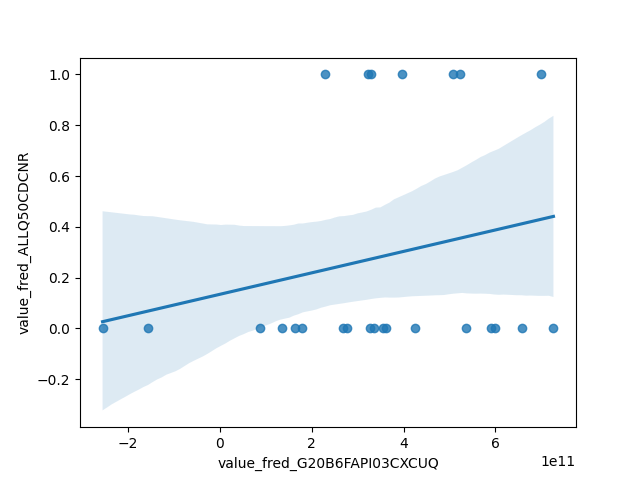
\includegraphics[scale = 0.9]{plots/plot_2024-12-24.png}
\caption{Regression Plot for 2024-12-24}
\end{figure}
\newpage
